\documentclass[aspectratio=169]{beamer}
\usetheme{Copenhagen}
\usepackage{amsmath, nccmath}
\usepackage{multirow}
\usepackage{xcolor,pifont}

\newcommand{\cmark}{\textcolor{green}{\text{\ding{51}}}}
\newcommand{\xmark}{\textcolor{red}{\text{\ding{55}}}}
\newcommand{\range}[2]{#1\!:\!#2} % range
\newcommand{\f}[2]{#1\!\left(#2\right)} % function

% Custom colors
\colorlet{royalblue}{blue!80!gray!80!green}
\colorlet{customgreen}{green!70!blue!70!gray}
\colorlet{navyblue}{blue!70!green!90!white}
\colorlet{redorange}{orange!60!red!70!gray}

% Colored text
\newcommand{\rtx}[1]{{\color{redorange}#1}}
\newcommand{\btx}[1]{{\color{royalblue}#1}}

\setbeamertemplate{navigation symbols}{}

\usepackage[utf8]{inputenc}
\usepackage{chari}

\title{PIPG for Rendezvous}
\author{Govind Chari}
\date{June 2023}
\institute{University of Washington}
% \logo{
\includegraphics[width=1.8cm]{img/seal_black.pdf}\hspace*{10cm}~
\includegraphics[height=2.5cm]{img/ACL_logo.png}}

\begin{document}
\begin{frame}
\titlepage
\begin{columns}
\begin{column}[c]{0.5\linewidth}
\begin{center}

\includegraphics[width=1.8cm]{img/seal_black.pdf}
\end{center}
\end{column}
\begin{column}[c]{0.5\linewidth}
\begin{center}
    \vspace{0.25cm}

\includegraphics[height=2.5cm]{img/ACL_logo.png}    
\end{center}
\end{column}
\end{columns}
\end{frame}

\logo{}

\begin{frame}{PIPG Overview}
    \textbf{PIPG} is
    \begin{itemize}
        \item A first order primal-dual conic optimizer
        \item Easily verifiable
        \item Factorization free
        \item Intuitive
        \item Warmstartable
        \item Very fast (3-7x faster than ECOS)
        \item Codable in an afternoon
        \item Supports infeasibility detection
    \end{itemize}
\end{frame}

\begin{frame}{Comparison with ECOS}
    \begin{center}
        \begin{tabular}{ |p{4cm}||p{1cm}|p{1cm}|}
            \hline
              & ECOS & PIPG \\
            \hline
            Warm Startable   & \xmark    &\cmark\\
            Verification Ease   & \xmark    &\cmark\\
            Factorization Free&   \xmark  & \cmark\\
            Understandable &   \xmark  & \cmark\\
            Implementation Ease&   \xmark  & \cmark\\
            Infeasibility Detection&   \cmark  & \cmark\\
            Tuning Free&   \cmark  & \xmark\\
            \hline
        \end{tabular}       
    \end{center}
\end{frame}

\begin{frame}{PIPG Algorithm}
    \vspace{-0.5cm}
    \begin{columns}[T]
        \begin{column}{.4\textwidth}
            \begin{block}{Optimization Problem}
                \begin{fleqn}
                    \begin{equation*}
                        \begin{aligned}
                        \min_{z} \quad & \frac{1}{2}z^{\top}Pz+q^\top z\\
                        \textrm{s.t.} \quad & Hz - h = 0\\
                          &z \in \D    \\
                        \end{aligned}
                    \end{equation*}
                \end{fleqn}
        \end{block}
        \end{column}
        \begin{column}{.6\textwidth}
            \begin{block}{Algorithm}
                    \begin{fleqn}
                            \begin{equation*}
                                z^{k+1} \gets \Pi_\D \brac{z^k - \alpha (Pz^k + q + H ^ \top w^k)}
                            \end{equation*}
                            \vspace*{-0.5cm}
                            \begin{equation*}
                                w^{k+1} \gets w^k + \beta(H(2z^{k+1}-z^k) - h)
                            \end{equation*}
                    \end{fleqn}
            \end{block}
        \end{column}
    \end{columns}
    \vspace{0.25cm}
    \begin{columns}[T]
        \begin{column}{.5\textwidth}
            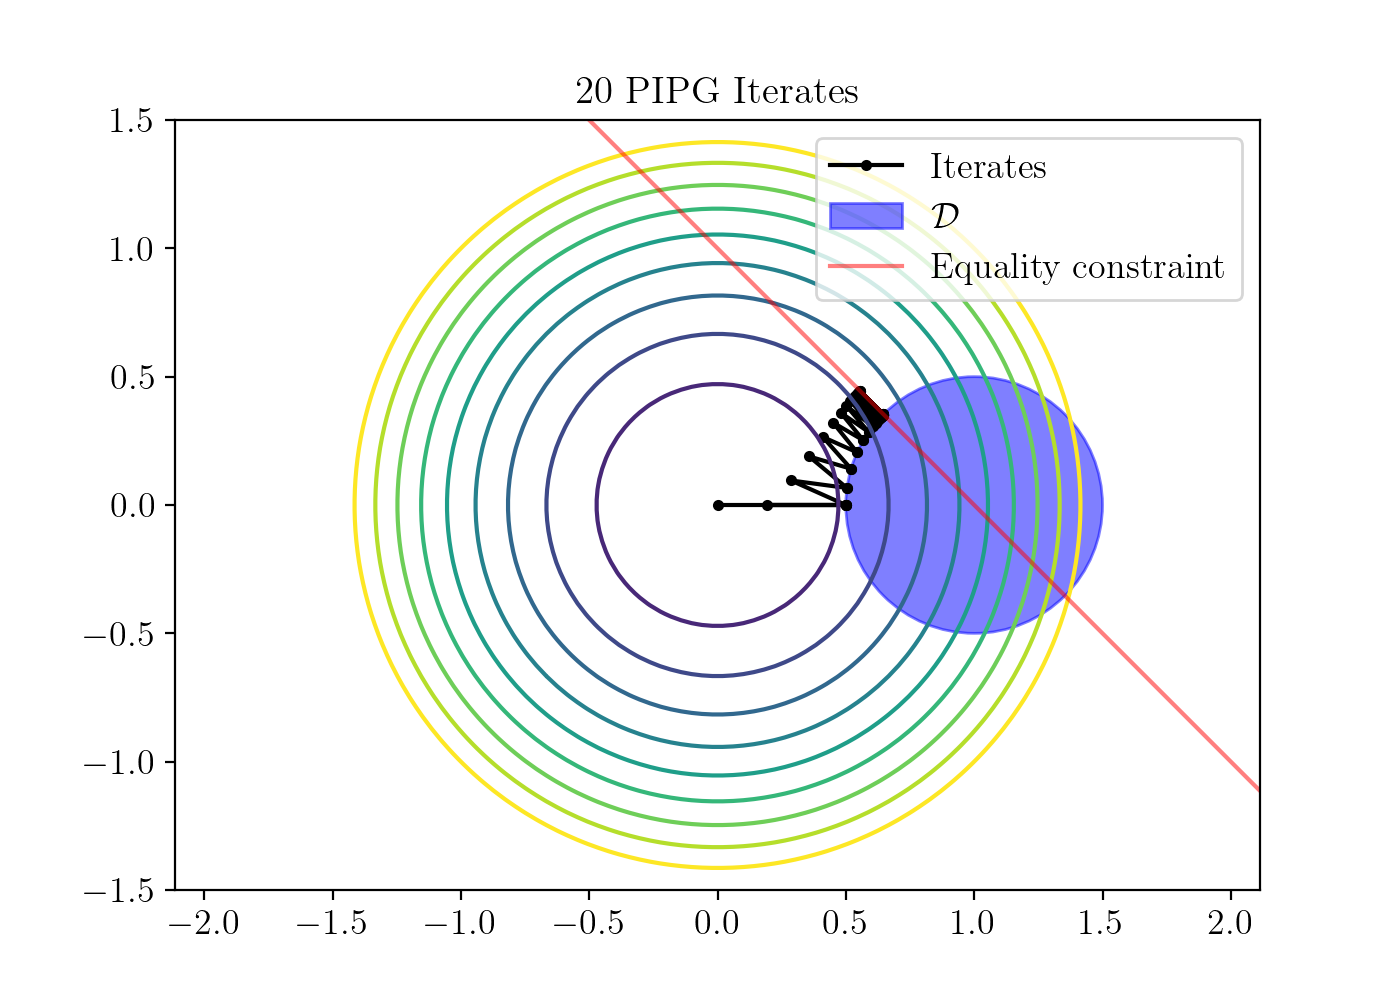
\includegraphics[width=6.75cm]{img/pipg_iterates.png}
        \end{column}
        \begin{column}{.5\textwidth}
            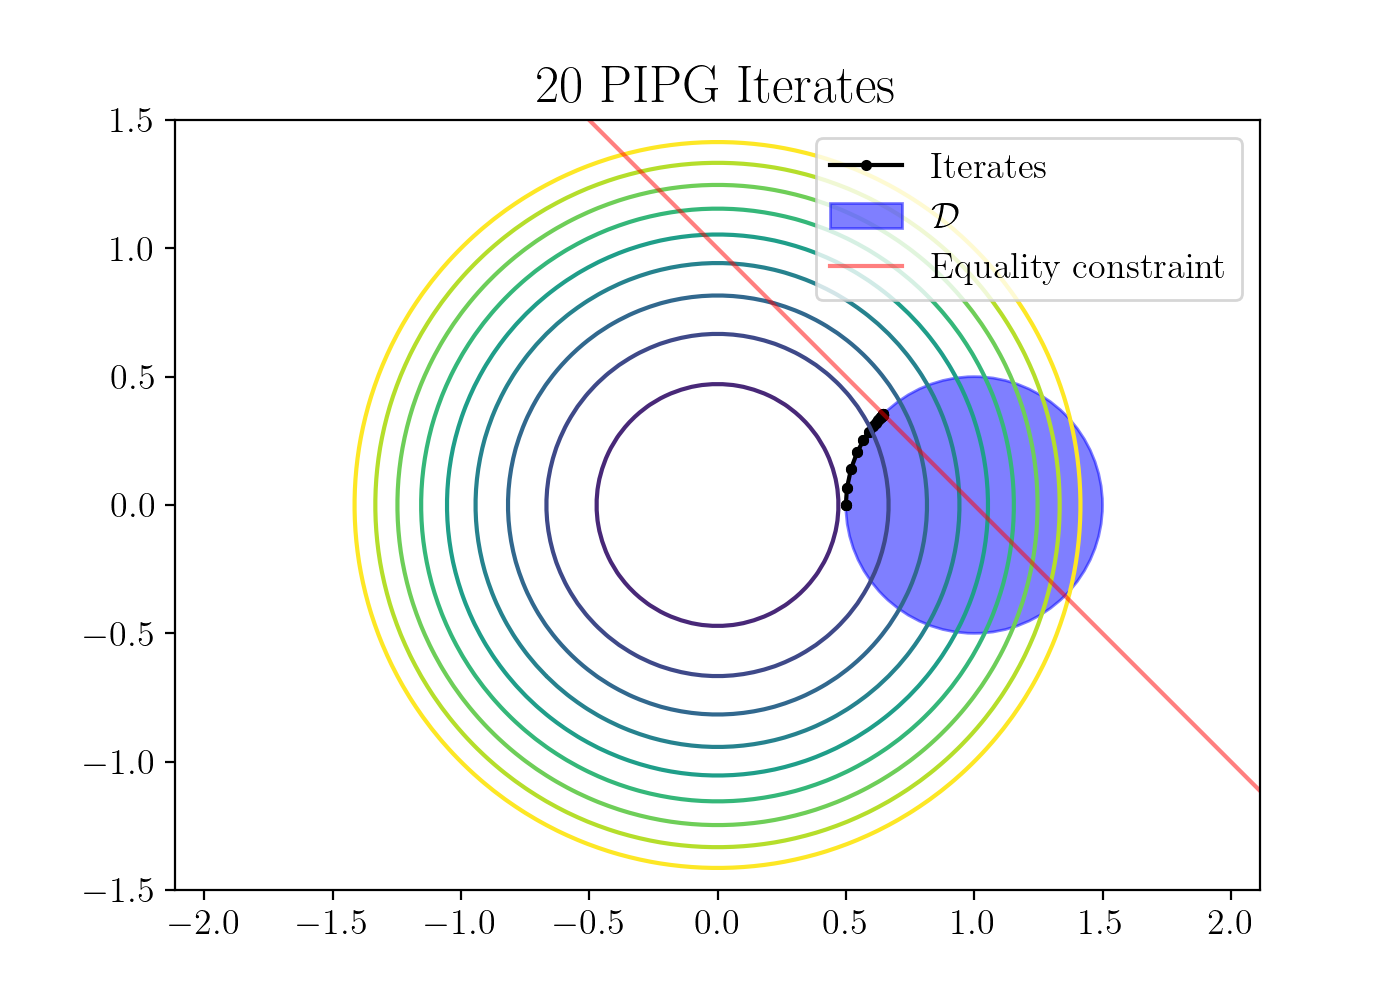
\includegraphics[width=6.75cm]{img/actual_pipg_iterates.png}
        \end{column}
    \end{columns}
\end{frame}

% \begin{frame}{Infeasibility Detection - Dual Infeasibility}
%     Dual Infeasibility Criteria: 
    
%     \[\lim_{k\to\infty} \|z^{k+1}-z^k\| \neq 0\]
%     \begin{columns}[T]
%         \begin{column}{.5\textwidth}
%             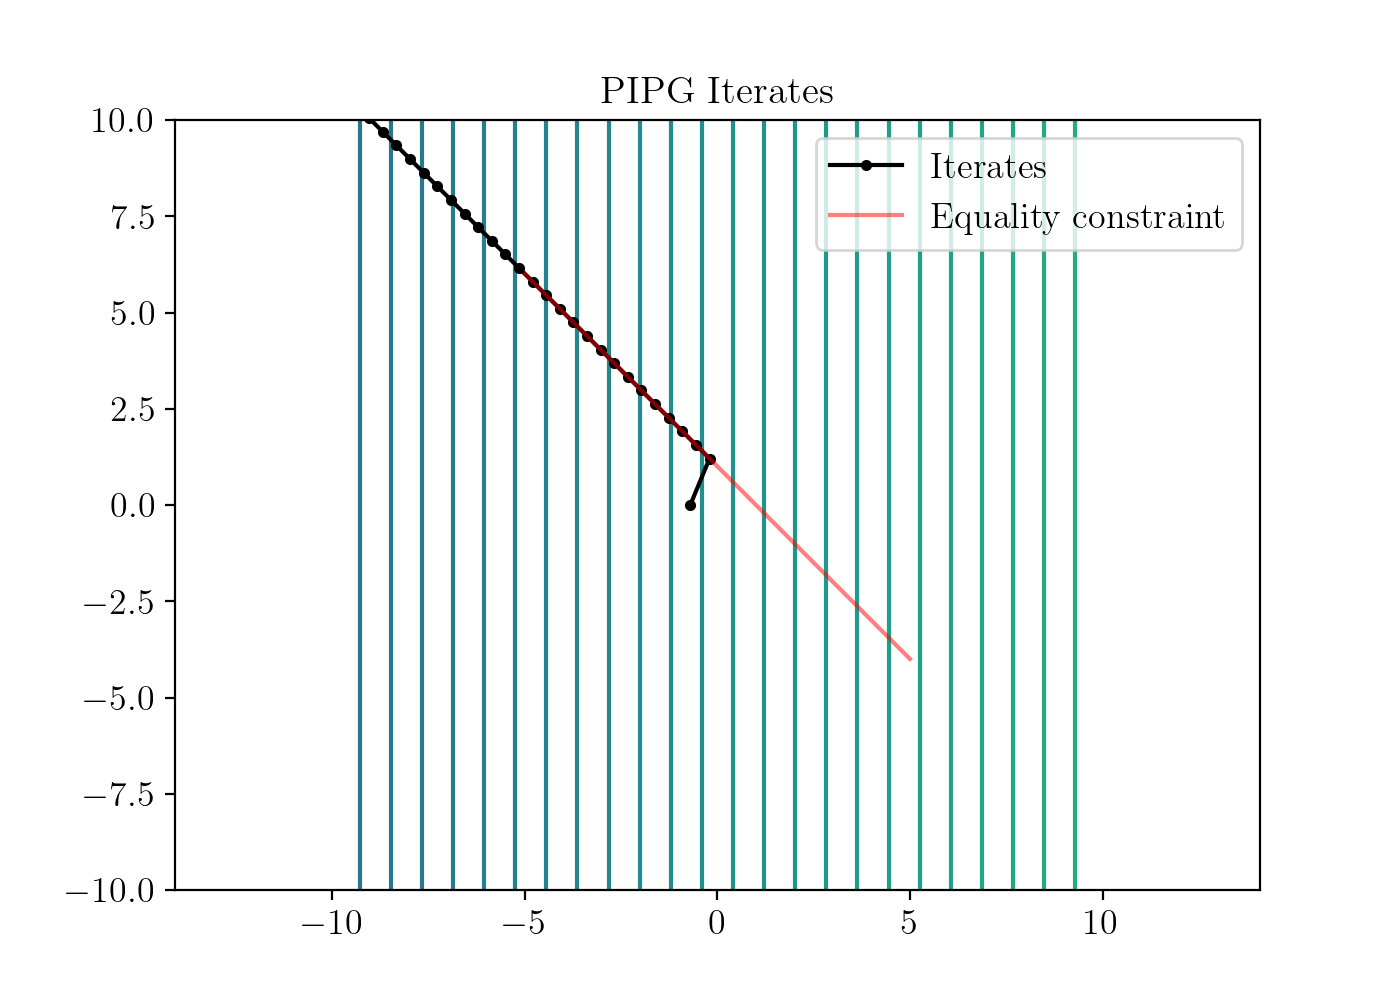
\includegraphics[width=7cm]{img/dual_infeas_pipg_iters.png}
%         \end{column}
%         \begin{column}{.5\textwidth}
%             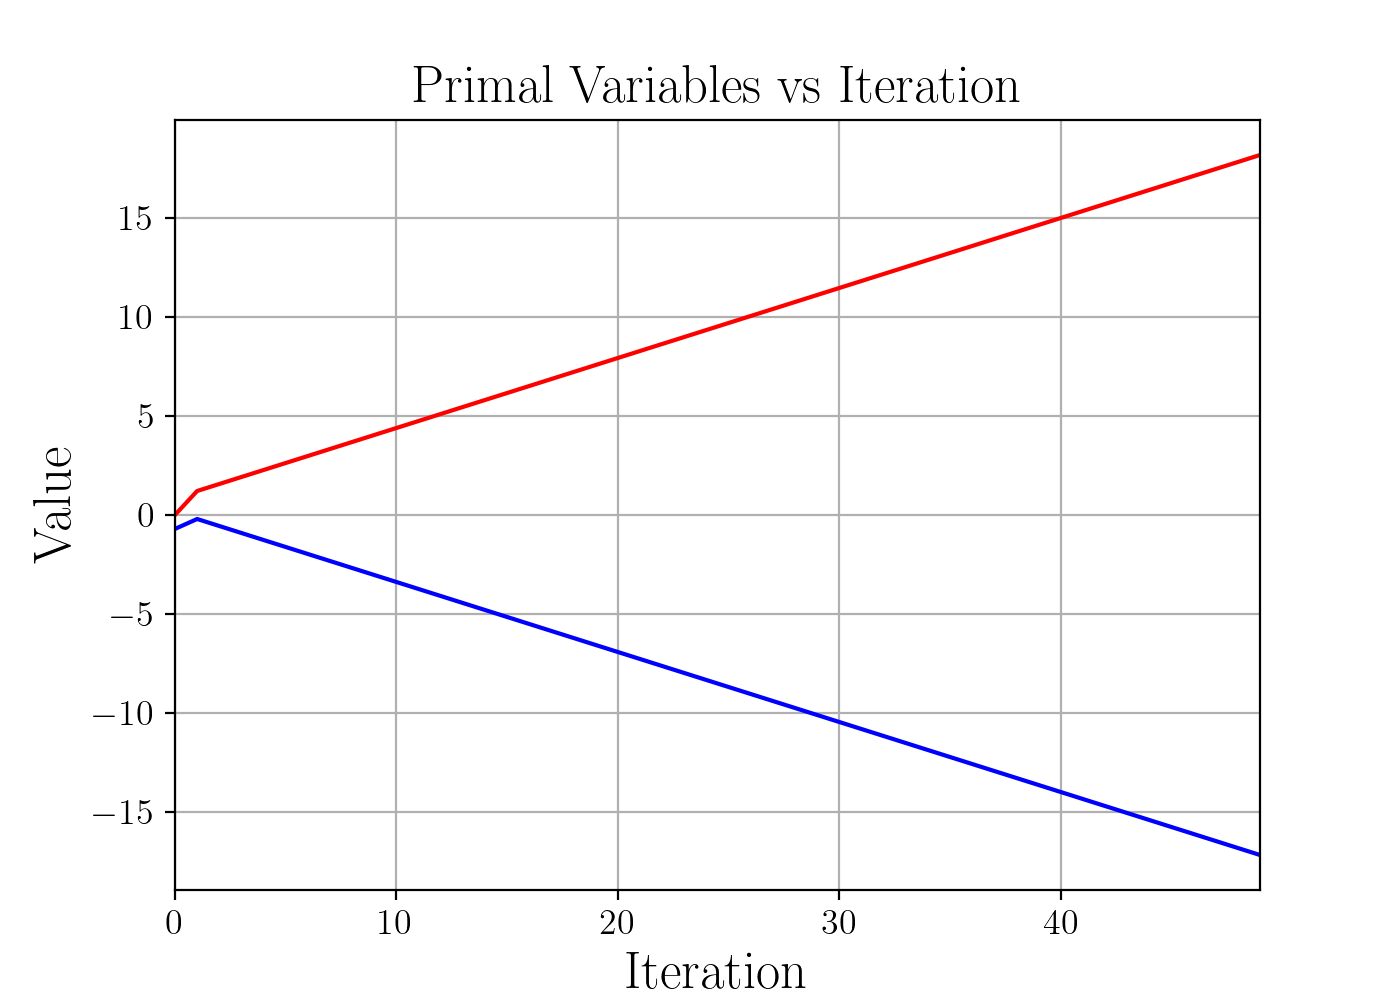
\includegraphics[width=7cm]{img/dual_infeas_prim_iters.png}
%         \end{column}
%     \end{columns}
% \end{frame}

\begin{frame}{Infeasibility Detection}
    Primal Infeasibility Criteria: 
    
    \[\lim_{k\to\infty} \|w^{k+1}-w^k\| \neq 0\]
    \begin{columns}[T]
        \begin{column}{.5\textwidth}
            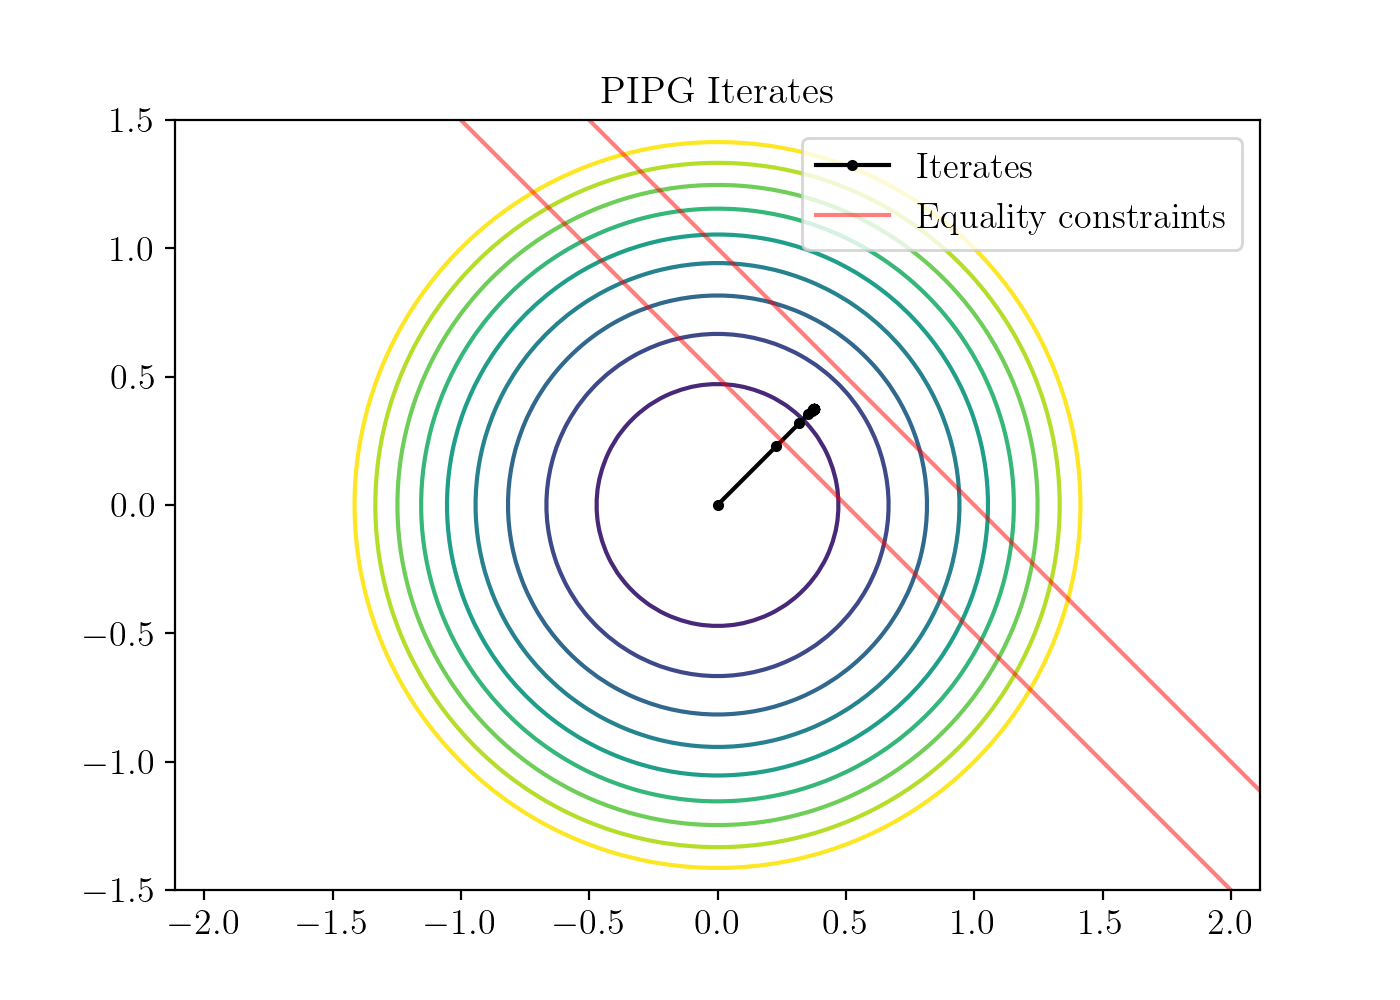
\includegraphics[width=7cm]{img/prim_infeas_pipg_iters.png}
        \end{column}
        \begin{column}{.5\textwidth}
            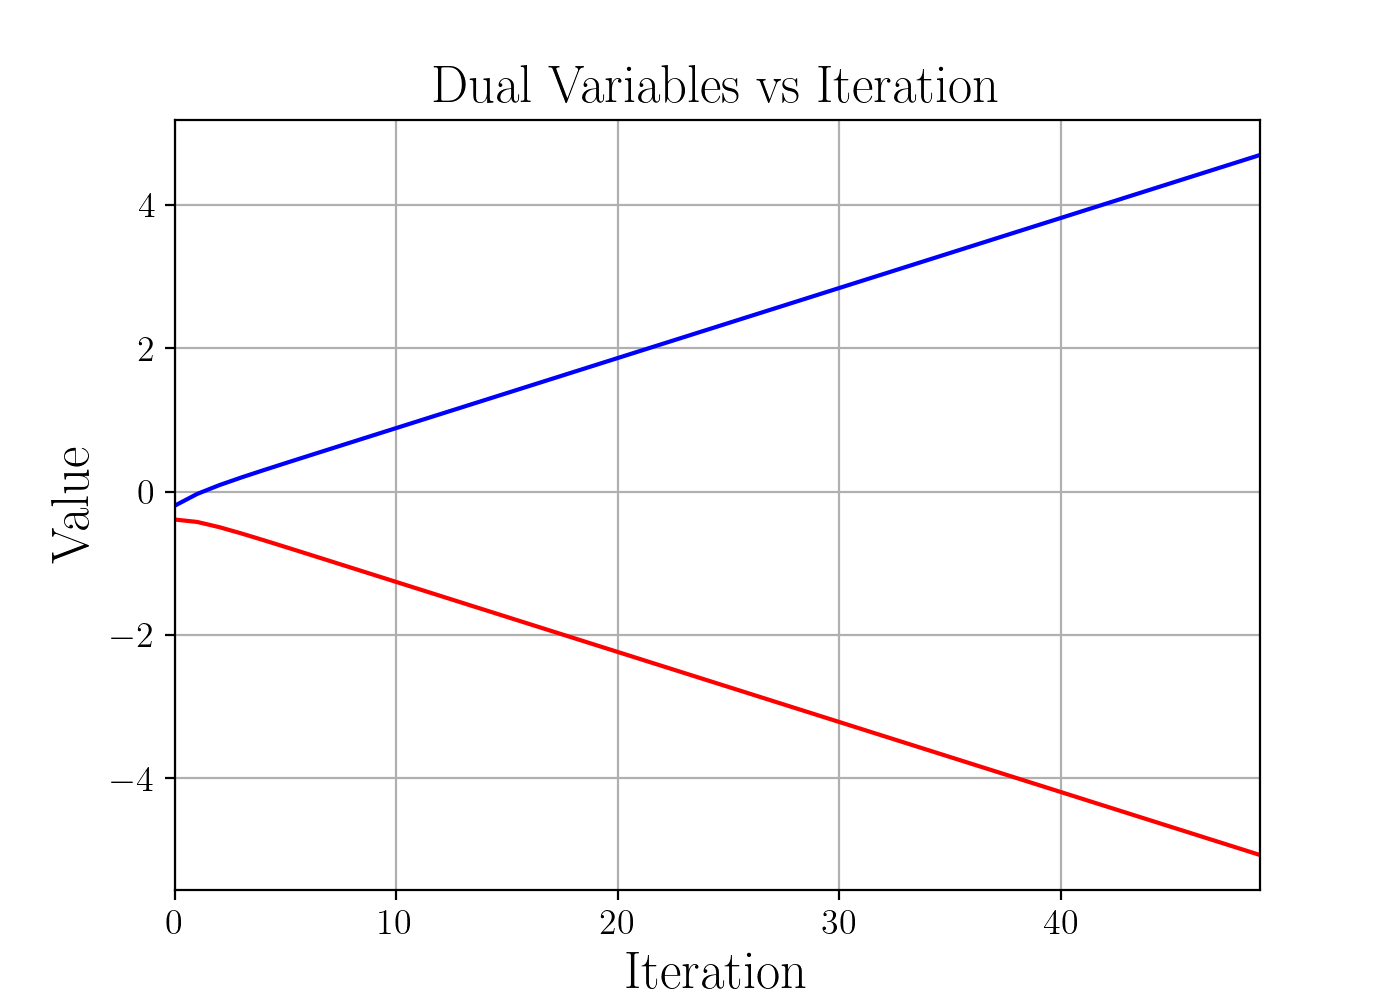
\includegraphics[width=7cm]{img/prim_infeas_dual_iters.png}
        \end{column}
    \end{columns}
\end{frame}
\begin{frame}{Structured Sparsity}
    \vspace{-0.8cm}
    \begin{columns}[T]
        \begin{column}{.55\textwidth}
            \begin{fleqn}
            \begin{equation*}
            \begin{aligned}
    \underset{x_t,u_t}{\operatorname{minimize}}~~~&~x_N^\top Q_N x_N+\sum_{t=1}^{N-1} x_t^\top Q_t x_t + u_t^\top R_t u_t\\
    \operatorname{subject~to}~&~x_{t+1} = A_t x_t + B_tu_t, \\
    &~x_t\in\mathbb{X}_t,~~u_t \in \mathbb{U}_t
            \end{aligned}
            \end{equation*}
            \end{fleqn}
            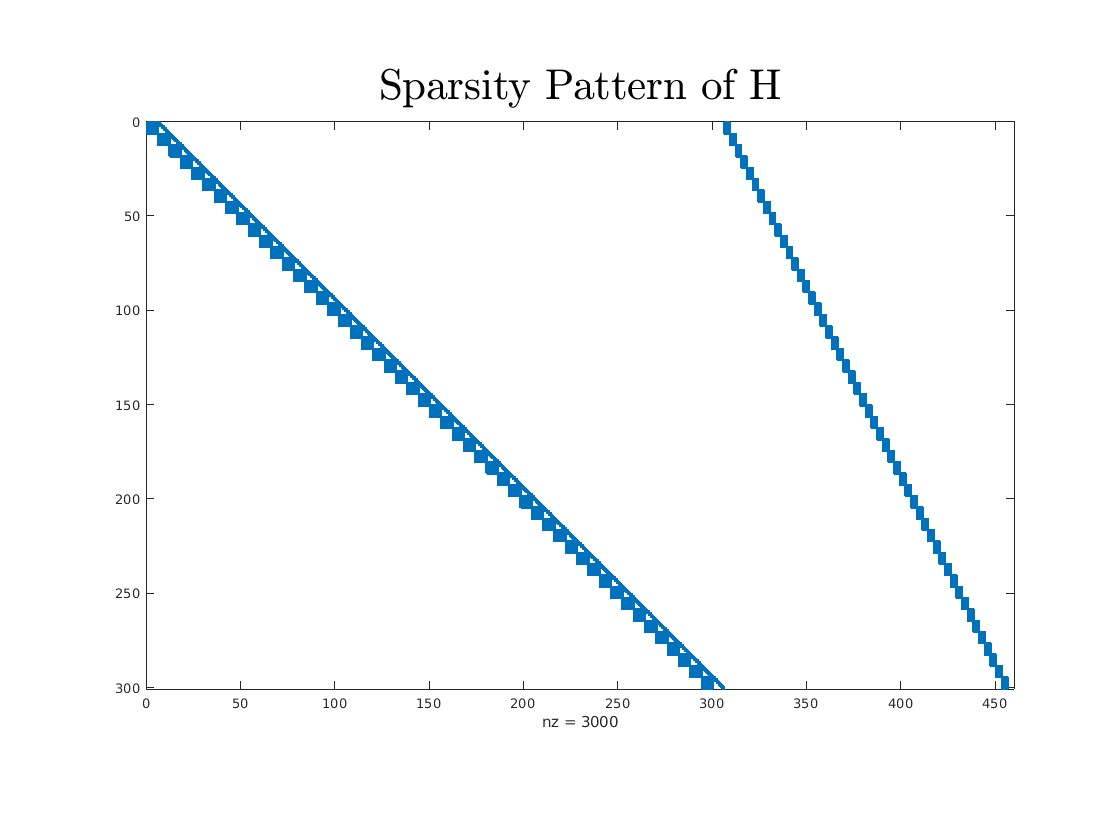
\includegraphics[width=7cm]{img/H_spy.jpg}
    \end{column}
        \begin{column}{.45\textwidth}
            \begin{fleqn}
            \begin{equation*}
            \begin{aligned}
        \underset{z}{\operatorname{minimize}}~~~&~\frac{1}{2}z^\top P z \\
        \operatorname{subject~to}~&~Hz-h=0,~ z\in\mathbb{D}
            \end{aligned}
            \end{equation*}
            \end{fleqn}

            \vspace{1.15cm}

        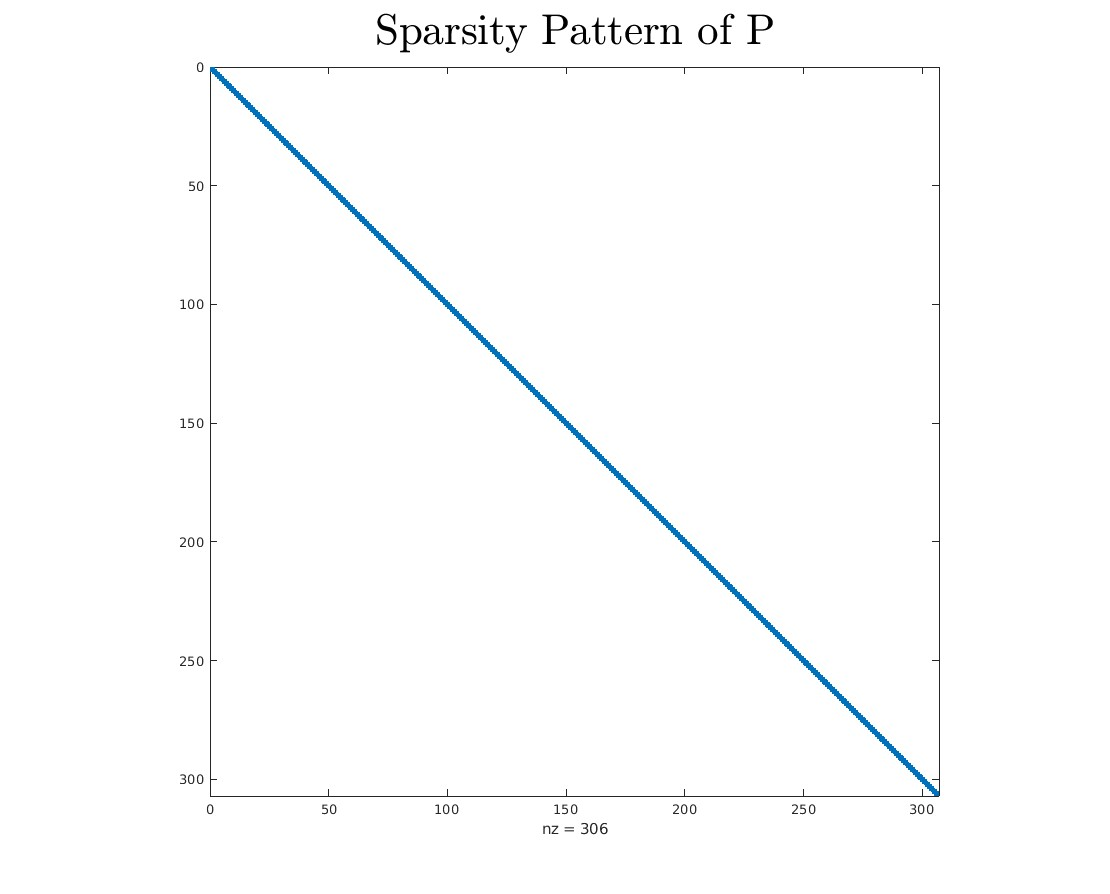
\includegraphics[width=6cm]{img/P_spy.jpg}
        \end{column}
    \end{columns}
\end{frame}

\begin{frame}{Customization: Structure Exploitation}
    \begin{columns}[T]
        \begin{column}{.5\textwidth}
            $\underbrace{\begin{bmatrix}
                A_{1} & & \\
                & \ddots & \\
                & & A_{K}
              \end{bmatrix}}_{\text{H}}
              \underbrace{
              \begin{bmatrix}
                x_{1}\\
                \vdots\\
                x_{K}
              \end{bmatrix}}_{\text{z}} = 
              \underbrace{
              \begin{bmatrix}
                A_{1}x_{1}\\
                \vdots\\
                A_{K}x_{K}
              \end{bmatrix}}_{\text{y}}$

              \vspace{0.5cm}


              We can compute $y=Hz$ subvector by subvector ($y_i = A_ix_i$) without constructing H and without using sparse-matrix vector multiplication.
            \end{column}
        \begin{column}{.5\textwidth}
            % 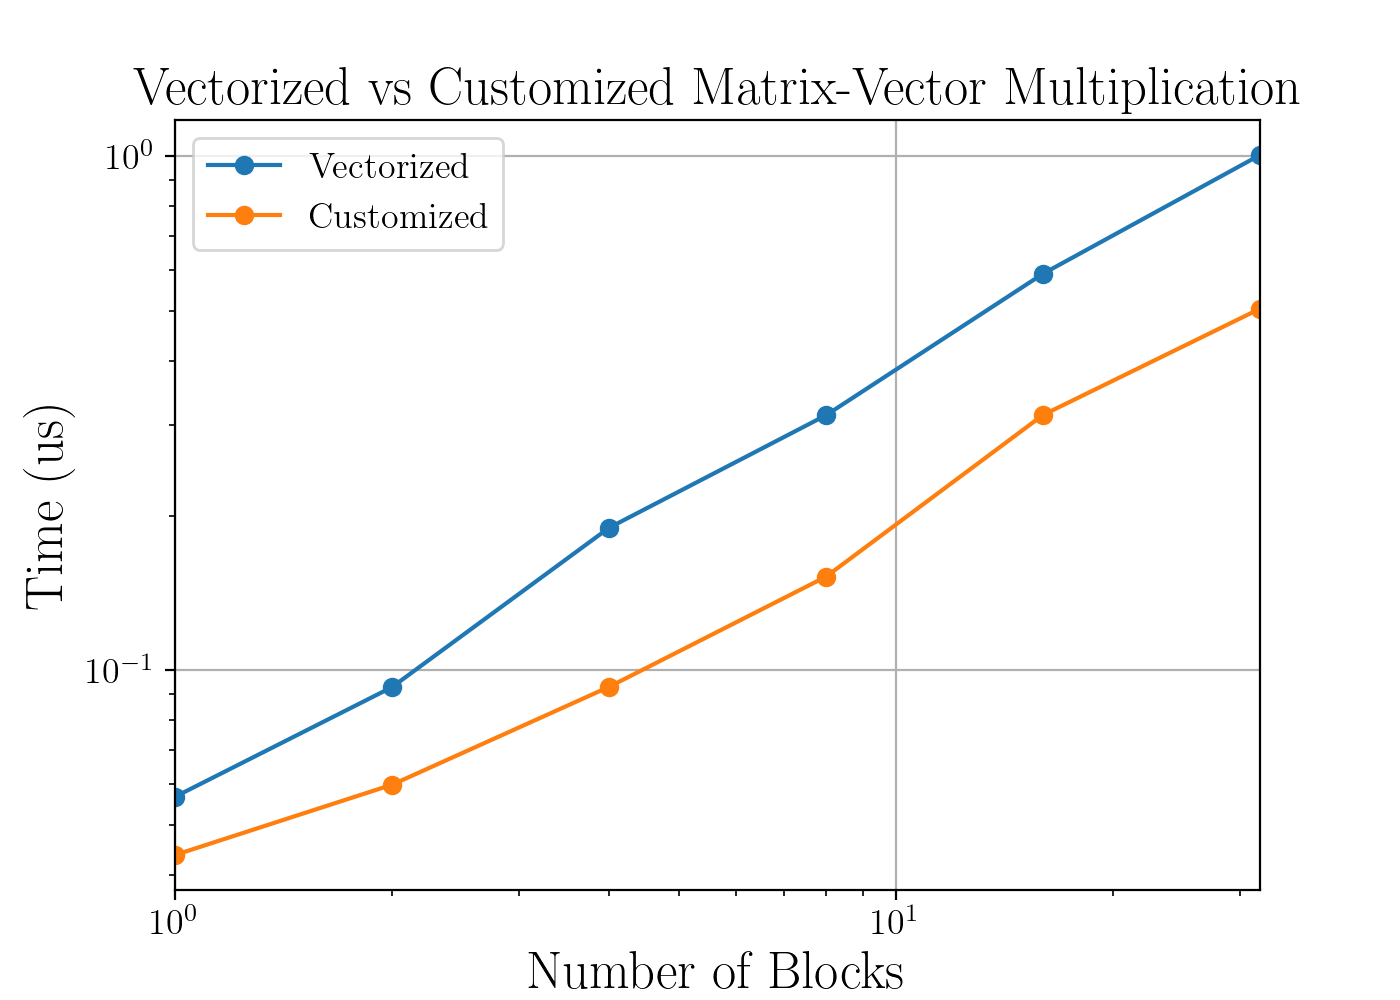
\includegraphics[width=0.75\textwidth]{img/customized.png}
            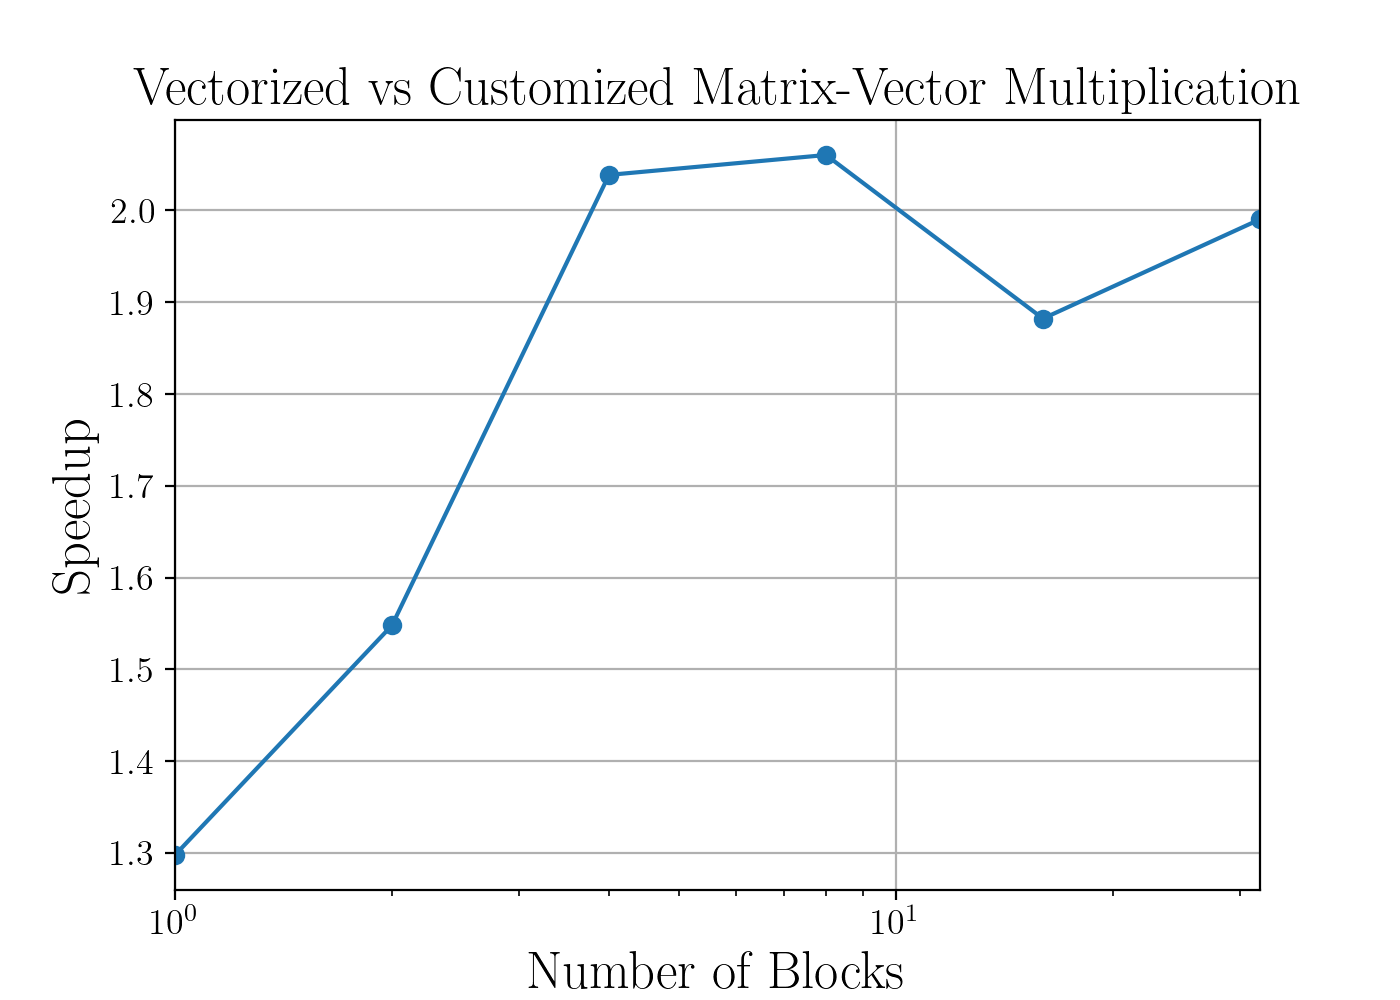
\includegraphics[width=\textwidth]{img/customized_speedup.png}

            \vspace{0.5cm}

            \begin{center}
                Customization can double structured matrix vector multiplication speed.
            \end{center}
        \end{column}
    \end{columns}
\end{frame}

\begin{frame}{Customization: PIPG}

    \vspace{-1cm}

    \begin{columns}[T]
        \begin{column}{0.6\textwidth}
            \begin{equation*}
                \begin{aligned}
        \underset{x_t,u_t}{\operatorname{minimize}}~~~&~x_N^\top Q_N x_N+\sum_{t=1}^{N-1} x_t^\top Q_t x_t + u_t^\top R_t u_t\\
        \operatorname{subject~to}~&~x_{t+1} = A_t x_t + B_tu_t, \\
        &~x_t\in\mathbb{X}_t,~~u_t \in \mathbb{U}_t
                \end{aligned}
                \end{equation*}  
                
                \vspace{1cm}

            $\begin{aligned}
                \rtx{w_t \gets {}} & \rtx{v_t+\beta (x_{t+1}-A_tx_{t}-B_tu_{t})} \\
                \btx{u_{t} \gets {}} & \btx{\Pi_{\mathbb{U}_t} [u_{t}-\alpha(R_tu_{t}-B_t^\top w_{t-1})]}\\
                \btx{x_t \gets {}} & \btx{\Pi_{\mathbb{X}_t}[x_t-\alpha(Q_tx_t+ w_{t-1}-A_t^\top w_{t})]}\\
                \rtx{v_t \gets {}} & \rtx{v_t +\beta (x_{t+1}-A_tx_{t}-B_tu_{t})}
            \end{aligned}$        
        \end{column}
        \begin{column}{0.4\textwidth}
            \begin{equation*}
                \begin{aligned}
            \underset{z}{\operatorname{minimize}}~~~&~\frac{1}{2}z^\top P z \\
            \operatorname{subject~to}~&~Hz-h=0,~ z\in\mathbb{D}
                \end{aligned}
                \end{equation*}
                
                \vspace{2cm}

            $\begin{aligned}
                \rtx{w \gets {}}   & \rtx{v + \beta(Hz-h)}\\
                \btx{z \gets {}}   & \btx{\Pi_{\mathbb{D}}[z - \alpha (Pz + H^\top w)]}\\
                \rtx{v \gets {}}   & \rtx{v + \beta(Hz-h)}            
            \end{aligned}$
    \end{column}
    \end{columns}
\end{frame}

\begin{frame}{Parsing}
    \begin{figure}
        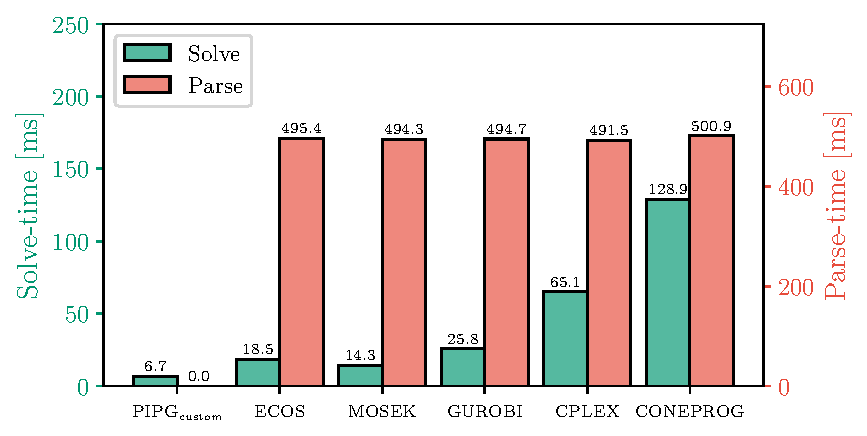
\includegraphics[width=0.90\textwidth]{img/bar_lqr_N30.pdf}
    \end{figure}

\vspace{0.25cm} 

{\footnotesize \color{gray} From Elango et al. \emph{SciTech 2022}}    
\end{frame}

% \begin{frame}{Customization}
%     \framesubtitle{Exploiting Structure}
%     {\small%
%     \begin{columns}
%     \begin{column}[c]{0.4\textwidth}
%     \begin{center}
%     $\begin{aligned}
%         \underset{z}{\operatorname{minimize}}~~~&~\frac{1}{2}z^\top P z \\
%         \operatorname{subject~to}~&~Hz-h=0,~ z\in\mathbb{D}
%     \end{aligned}$
%     \vspace{1.8cm}
%     \uncover<3->{%
%     $\begin{aligned}
%         \rtx{w \gets {}}   & \rtx{v + \beta(Hz-h)}\\
%         \btx{z \gets {}}   & \btx{\Pi_{\mathbb{D}}[z - \alpha (Pz + H^\top w)]}\\
%         \rtx{v \gets {}}   & \rtx{v + \beta(Hz-h)}
%     \end{aligned}$}
%     \end{center}
%     \end{column}
%     \begin{column}{0.04\textwidth}
%     \begin{center}
%         \vspace{0.8cm}
%         \uncover<2->{$\rightarrow$}
%         \vspace{2.7cm}
%         \uncover<4->{$\rightarrow$}
%         \vspace{1cm}
%     \end{center}
%     \end{column}
%     \begin{column}[c]{0.55\textwidth}
%     \begin{center}
%     \uncover<2->{%
%     $\begin{aligned}
%         \underset{x_t,u_t}{\operatorname{minimize}}~~~&~x_N^\top Q_N x_N+\sum_{t=1}^{N-1} x_t^\top Q_t x_t + u_t^\top R_t u_t\\
%         \operatorname{subject~to}~&~x_{t+1} = A_t x_t + B_tu_t, \\
%         &~x_t\in\mathbb{X},~~u_t \in \mathbb{U}
%     \end{aligned}$}
%     \vspace{1cm}
%     \uncover<4>{%
%     $\begin{aligned}
%         \rtx{w_t \gets {}} & \rtx{v_t+\beta (x_{t+1}-A_tx_{t}-B_tu_{t})} \\
%         \btx{u_{t} \gets {}} & \btx{\Pi_{\mathbb{U}} [u_{t}-\alpha(R_tu_{t}-B_t^\top w_{t-1})]}\\
%         \btx{x_t \gets {}} & \btx{\Pi_{\mathbb{X}}[x_t-\alpha(Q_tx_t+ w_{t-1}-A_t^\top w_{t})]}\\
%         \rtx{v_t \gets {}} & \rtx{v_t +\beta (x_{t+1}-A_tx_{t}-B_tu_{t})}
%     \end{aligned}$}
%     \end{center}
%     \end{column}
%     \end{columns}}
% \end{frame}

\begin{frame}{Continuous-time Nonconvex Problem}
    \begin{equation*}
        % \small
            \begin{aligned}
            \underset{t_{f},\,{x}(t), {u}(t)}{\text{minimize}} &
            && \int_{0}^{t_f} \|\f{u}{t}\|_2^2 \,dt \\
            \text{subject to} &
            && \forall t \in [0, t_f) \\
            \fbox{\text{CW Dynamics}} &&& {\f{\dot{{x}}}{t}} = \f{f}{{\f{{x}}{t}}, {\f{{u}}{t}}} \\
            \fbox{\text{Max delta-v}} &&& \|\f{u}{t}\|_2 \le u_{\max}\\
            \fbox{\text{Keepout Zone}} &&& 
            \|{r}(t)-r_c\|_2 \geq \rho \hphantom{\qquad\qquad} \\
            \fbox{\text{Max Speed}}
            &&& \|{v}(t)\|_2 \leq v_{\mathrm{max}} \\
            \fbox{\text{Initial Conditions}}
            &&& {r}(0) = {r}_i \\
            &&& {v}(0) = {v}_i \\
            \fbox{\text{Terminal Conditions}}
            &&& {r}(t_f) = {0}_{3 \times 1} \\
            &&& {v}(t_f) = {0}_{3 \times 1} \\
            \end{aligned}
        \end{equation*}
\end{frame}
\begin{frame}{Sequential Convex Programming (SCP)}
    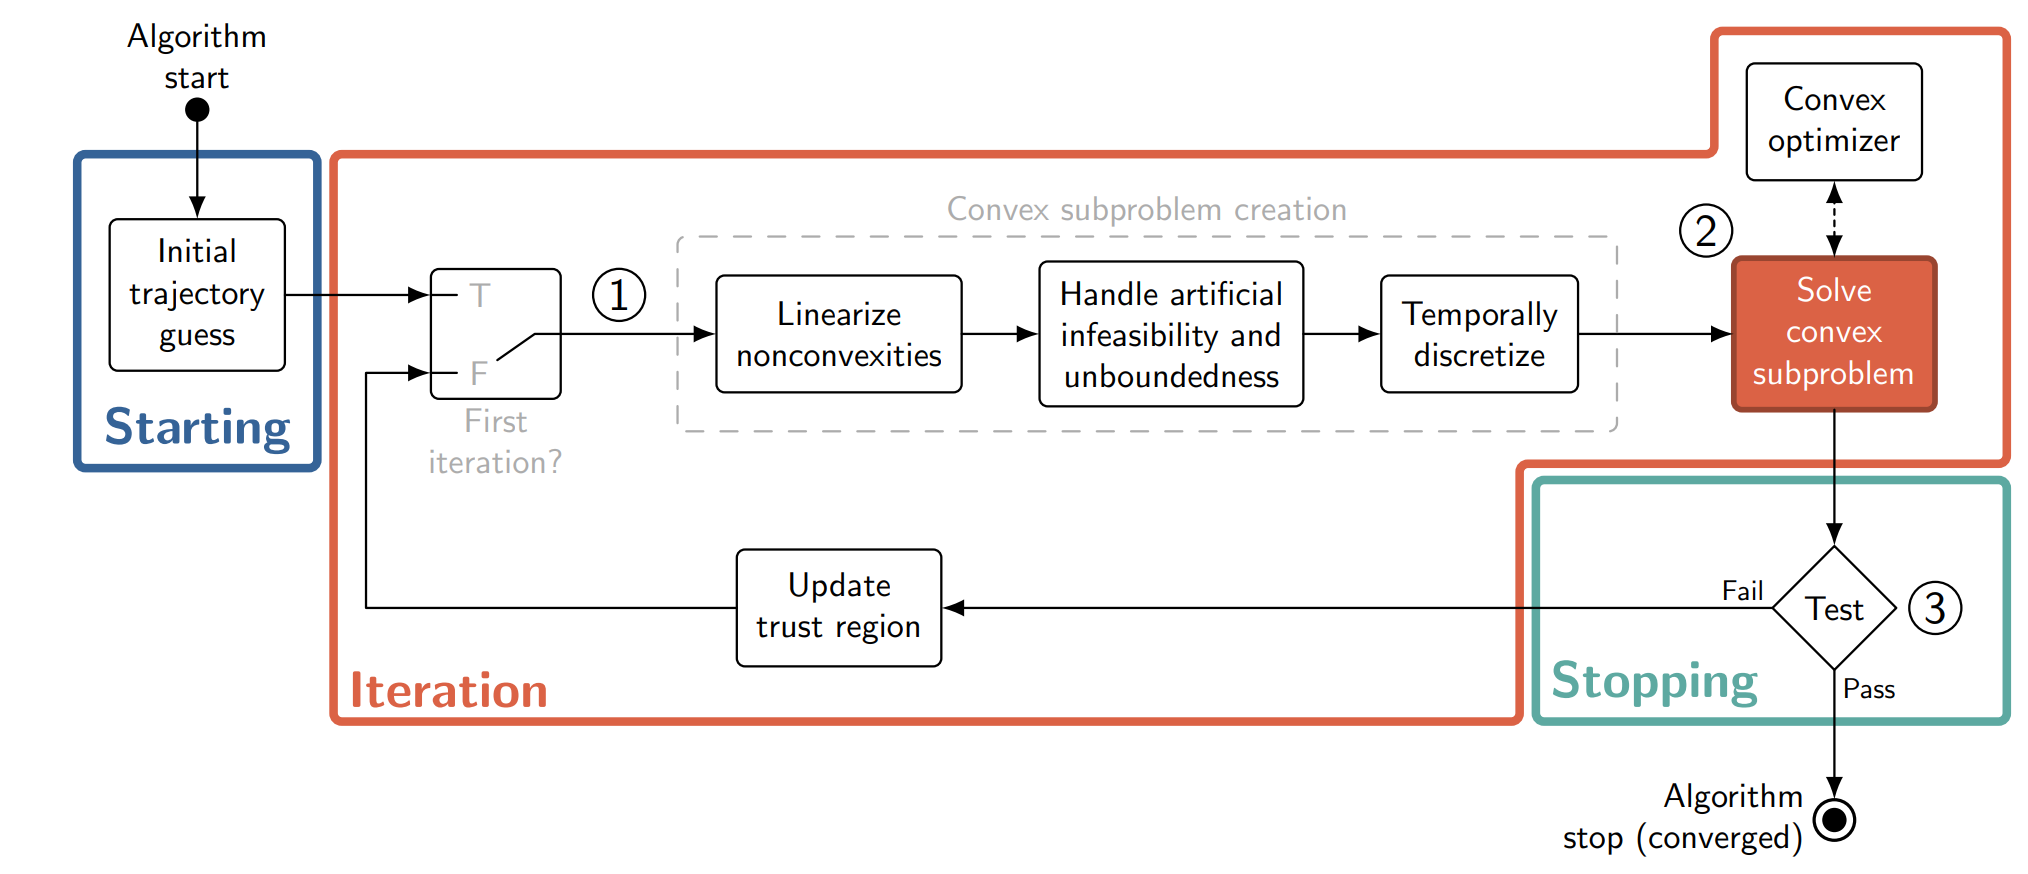
\includegraphics[width=\linewidth]{img/scp_block_diagram_csm.png}
    {\footnotesize \color{gray} From Malyuta et al. \emph{IEEE CSM 2022}}    
\end{frame}
\begin{frame}{Discrete-time Convex Subproblem}
    \begin{center}

    \resizebox{1.0\linewidth}{!}{$\begin{aligned}
            \underset{\sigma,\,x, u}{\text{minimize}} &
            && \sum_{k=1}^{K-1}\|u_k\|_2^2 + w_{tr}\left( \sum_{k=1}^{K}\|x_k-\hat{x}_k\|_2^2 + \sum_{k=1}^{K-1}[\|u_k-\hat{u}_k\|_2^2 + (\sigma_k-\hat{\sigma}_k)^2]\right) + w_{{vc}}\|\nu^{{c}}\|_1 + w_{{vb}}\sum_{k=1}^{K}\nu_k^b \\
            \text{subject to} &
            && \forall k \in [1, K] \\
            \fbox{\text{Discrete Dynamics}} &&& {x_{k+1}} = A_kx_k + B_ku_k + S_k\sigma_k + c_k + \nu_k^c \\
            \fbox{\text{Dilation Constraints}} &&& \sigma_{\min} \leq \sigma_k \le \sigma_{\max}\\
            \fbox{\text{Max delta-v}} &&& \|u_k\|_2 \le u_{\max}\\
            \fbox{\text{Keepout Zone}} &&& 
            \|\hat{r}_k-r_c\|_2 + \left(\frac{\hat{r}_k-r_c}{\|\hat{r}_k-r_c\|_2}\right)^\top (r_k-\hat{r}_k) + \nu_k^b \geq \rho \hphantom{\qquad\qquad} \\
            &&& \nu_k^b \geq 0 \\
            \fbox{\text{Max Speed}}
            &&& \|v_k\|_2 \leq v_{\mathrm{max}} \\
            \fbox{\text{Initial Conditions}}
            &&& {r}(1) = {r}_i \\
            &&& {v}(1) = {v}_i \\
            \fbox{\text{Terminal Conditions}}
            &&& {r}(K) = {0}_{3 \times 1} \\
            &&& {v}(K) = {0}_{3 \times 1} \\
            \end{aligned}$}

        \end{center}
\end{frame}
\begin{frame}{Trajectory}
    \vspace{-0.25cm}
    \begin{columns}[T]
        \begin{column}{.5\textwidth}
            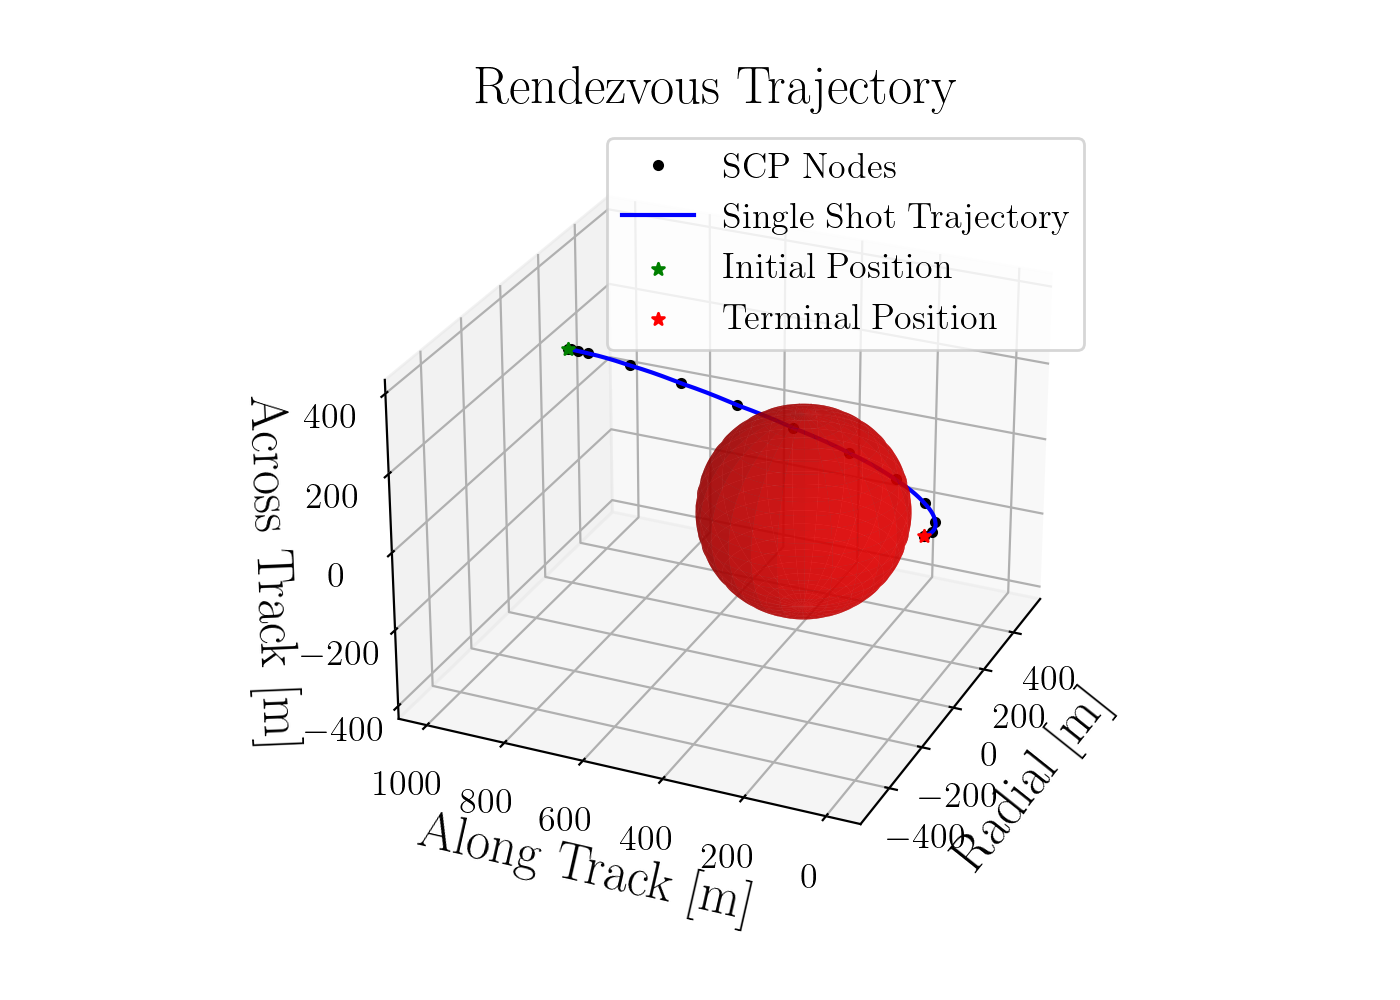
\includegraphics[width=8cm]{img/traj_side.png}
        \end{column}
        \begin{column}{.5\textwidth}
            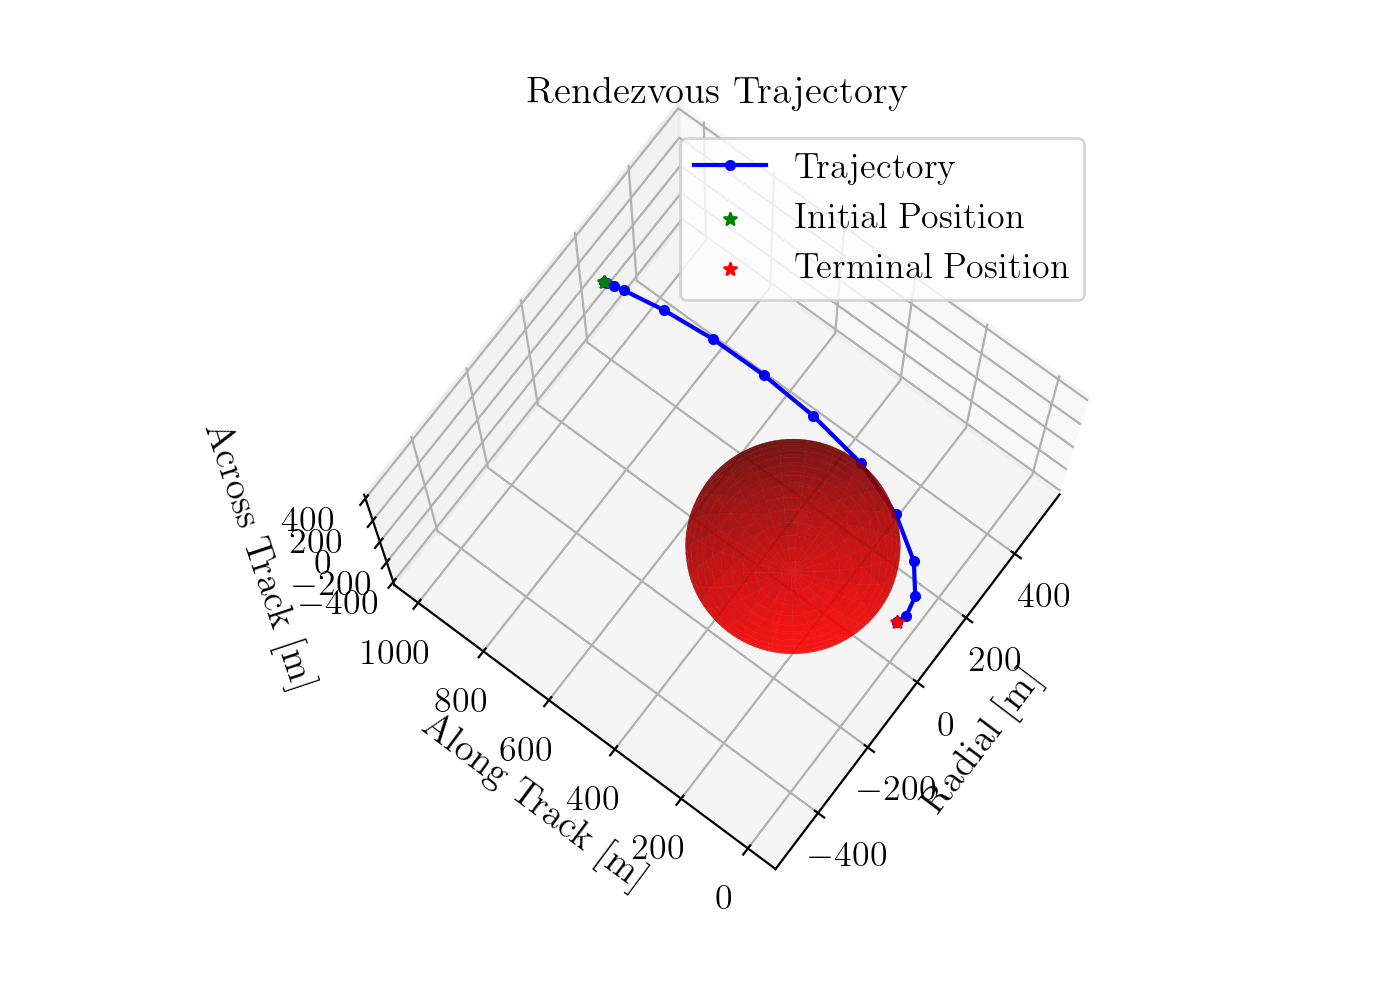
\includegraphics[width=8cm]{img/traj_top.png}
        \end{column}
    \end{columns}
\end{frame}

\begin{frame}{Trajectory}
    \vspace{-0.25cm}
    \begin{columns}[T]
        \begin{column}{.5\textwidth}
            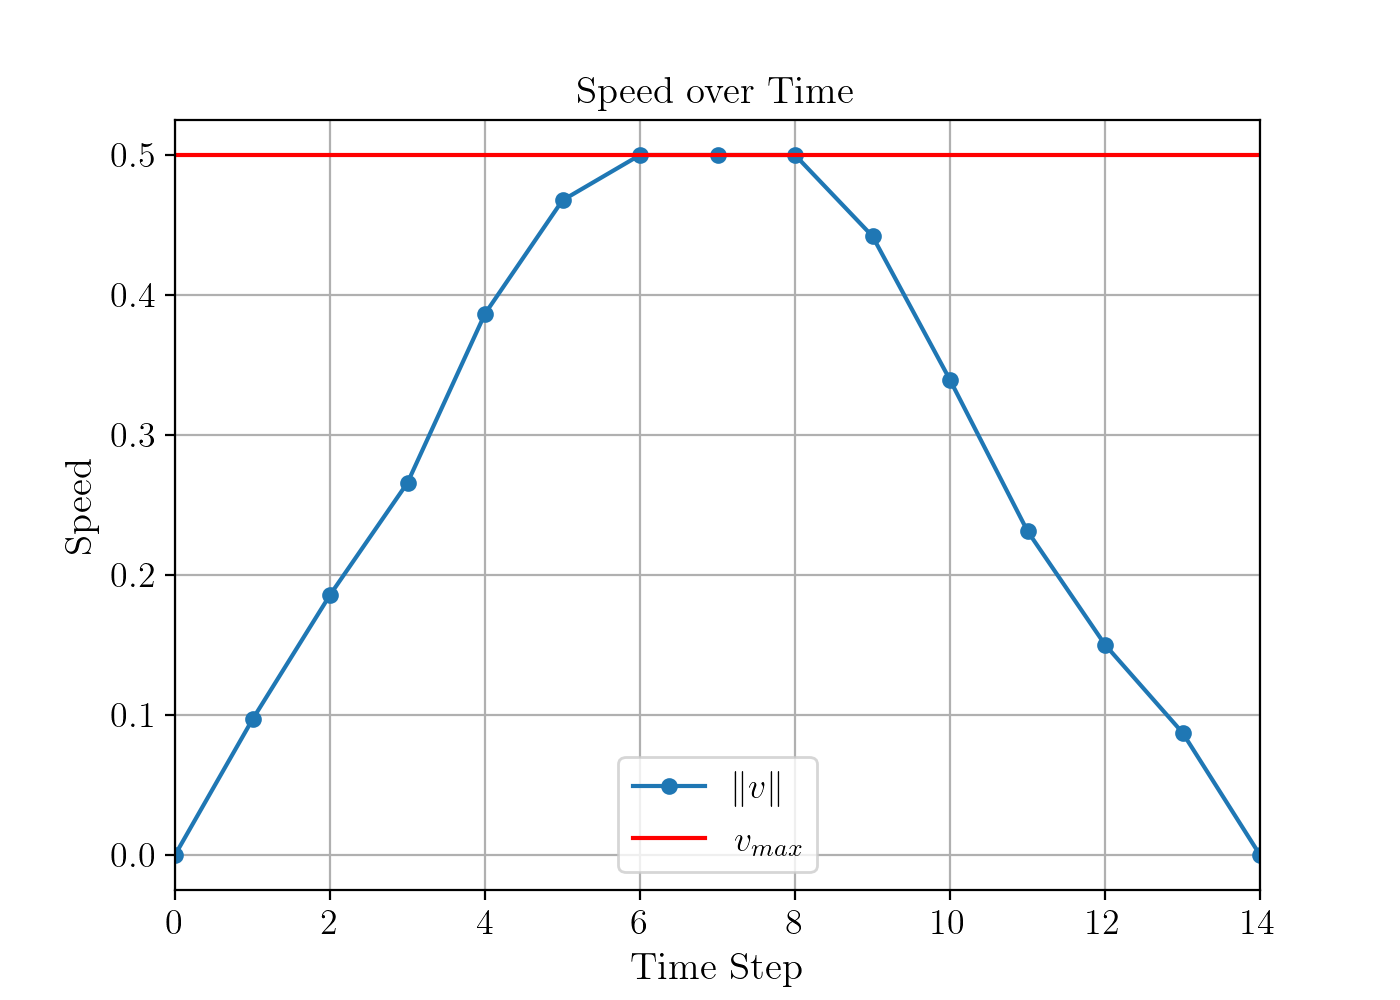
\includegraphics[width=8cm]{img/speed.png}
        \end{column}
        \begin{column}{.5\textwidth}
            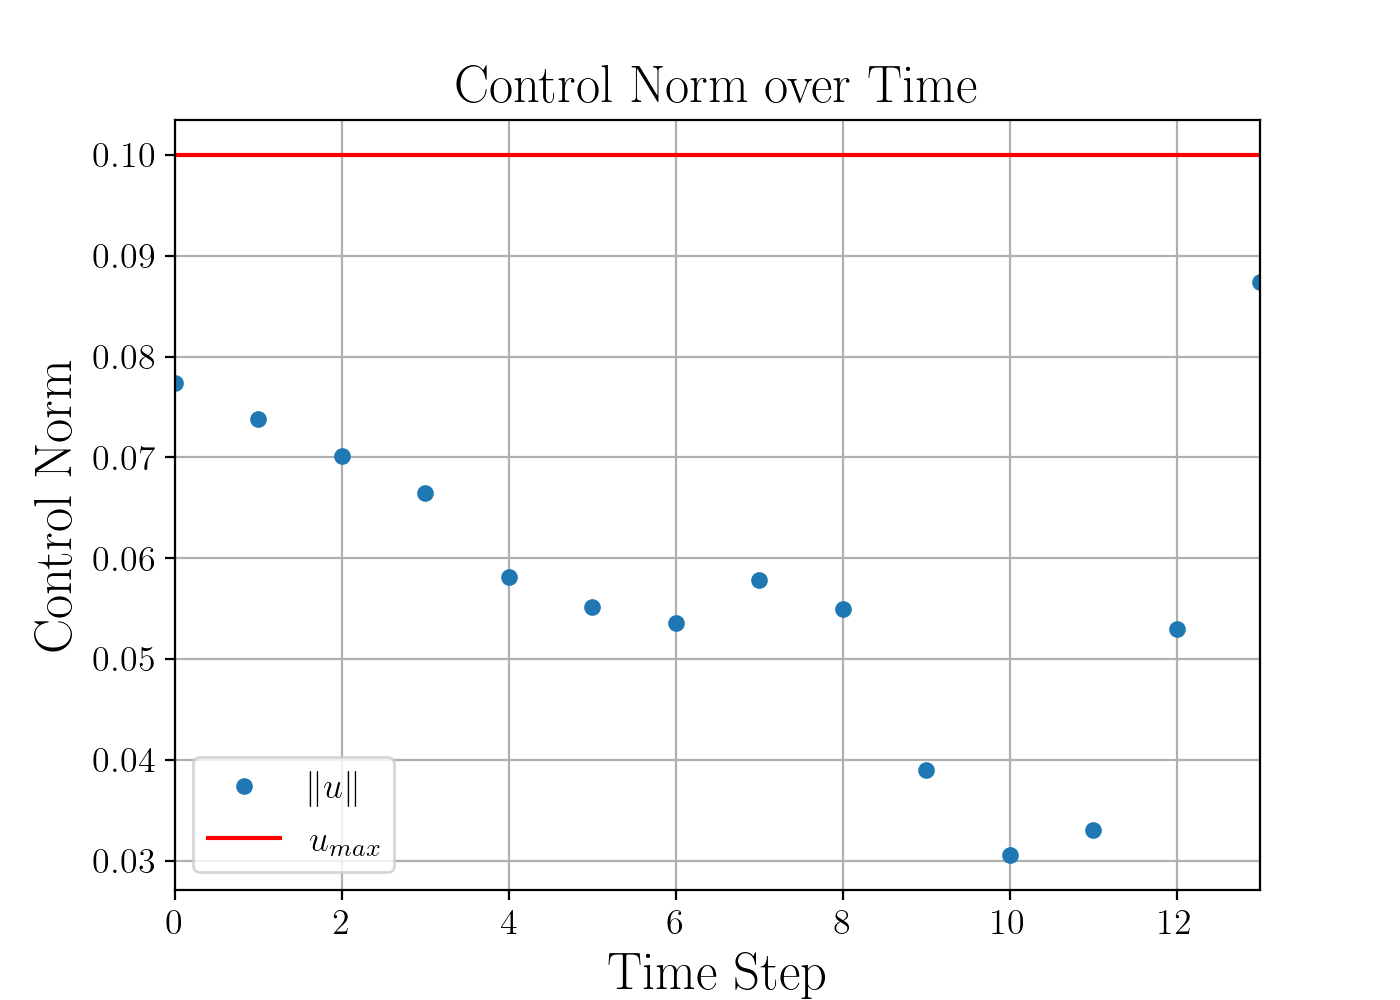
\includegraphics[width=8cm]{img/control.png}
        \end{column}
    \end{columns}
\end{frame}
\begin{frame}{Speed Results}

    % \vspace{-1cm}

    \begin{columns}[T]
        \begin{column}{.6\textwidth}
            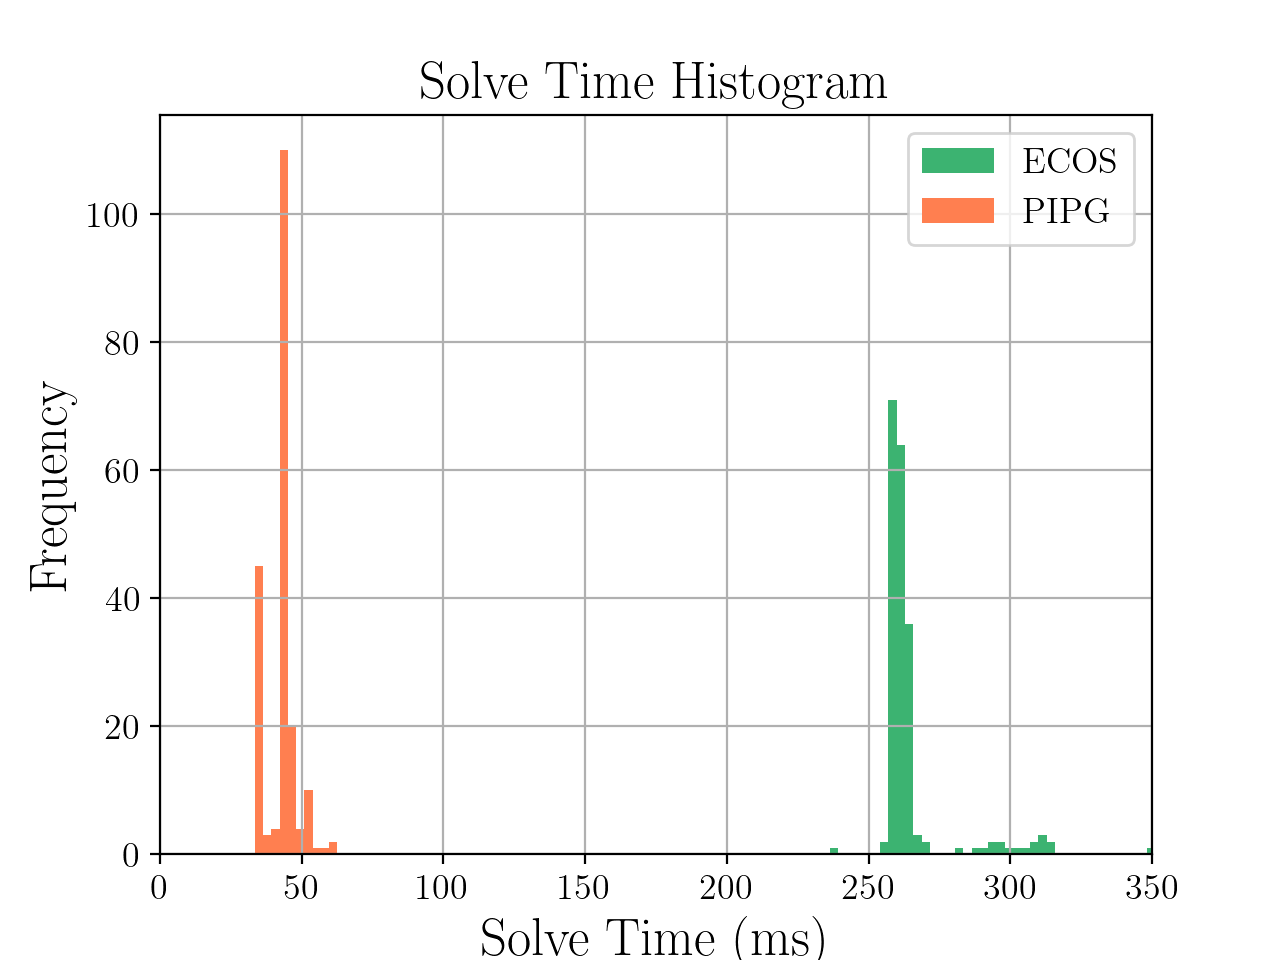
\includegraphics[width=\linewidth]{img/solve_speed.png}\begin{center}
                {200 runs, 3 millisecond bins}
            \end{center}
        \end{column}
        \begin{column}{.4\textwidth}
            \begin{center}
                \resizebox{1.0\linewidth}{!}{

                \begin{tabular}{|p{2cm}||p{1.5cm}|p{1.5cm}|}
                    \hline
                      & ECOS & PIPG \\
                    \hline
                    Mean   & 261ms    & \textbf{42ms}\\
                    Median &   267ms  & \textbf{44ms}\\
                    STD &   23ms  & \textbf{5ms}\\
                    \hline
                \end{tabular} }

                \vspace{0.5cm}

            \end{center} 
            
            PIPG is \textbf{\textcolor{red}{6.25x}} faster even without customization

        \end{column}
    \end{columns}
\end{frame}
\begin{frame}{Summary}
    \begin{columns}[T]
        \begin{column}{0.35\textwidth}
            \textbf{PIPG} is
            \begin{itemize}
                \item Easy to understand
                \item Easy to verify
                \item Easy to implement
                \item Faster than ECOS
            \end{itemize}        
        \end{column}
        \begin{column}{0.65\textwidth}
            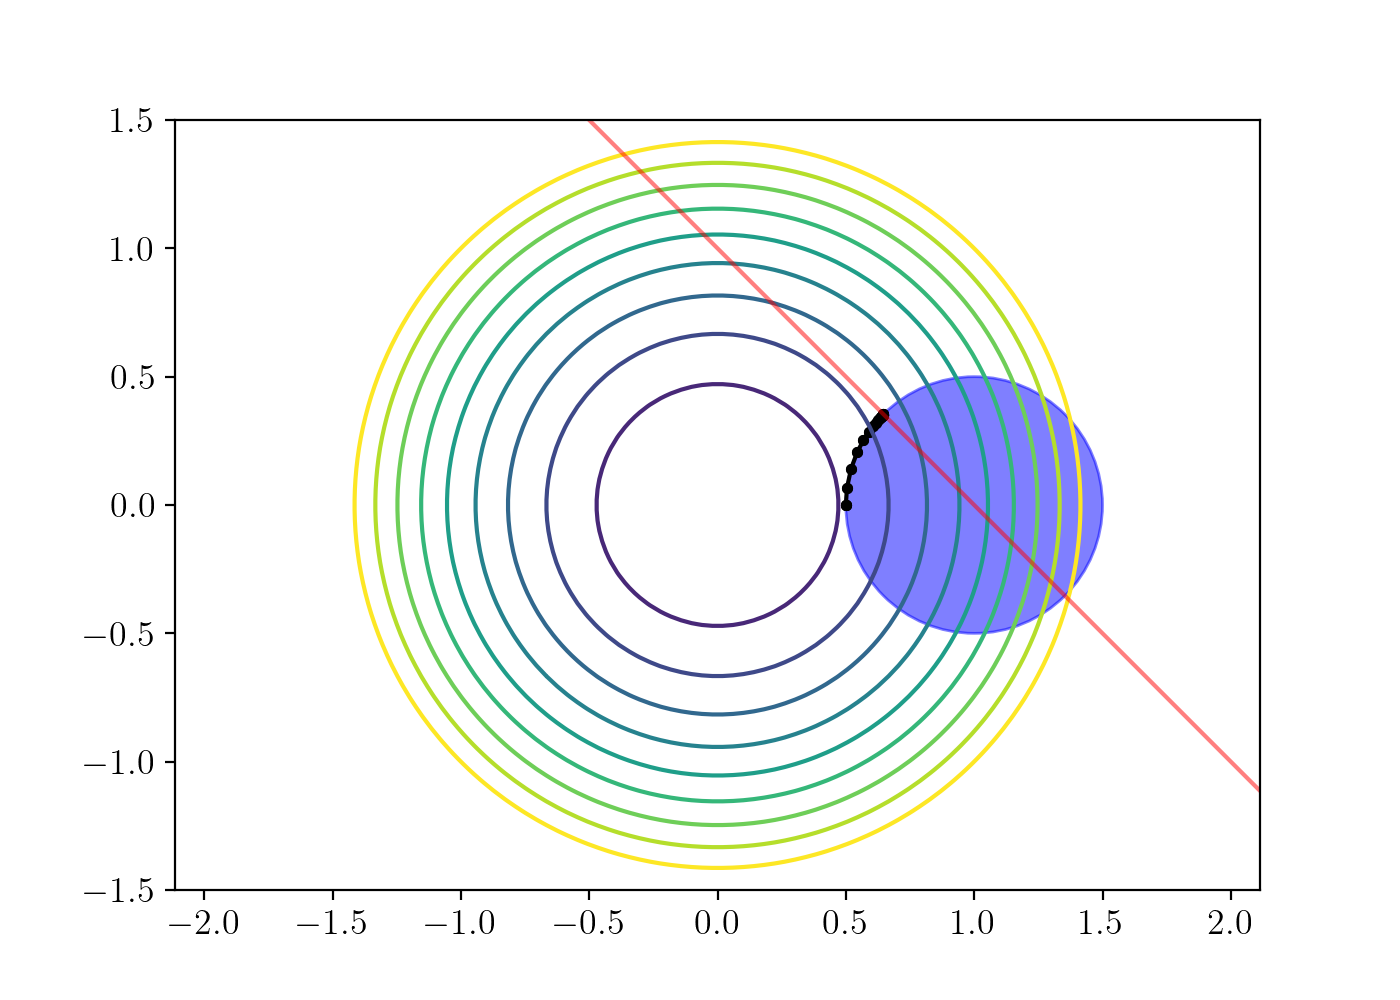
\includegraphics[width=\textwidth]{img/pipg_candy.png}
        \end{column}
    \end{columns}
\end{frame}

\end{document}